\subsection{Działanie programu}\label{sub:dzialanie programu}
\paragraph{}

Podstawowymi aktywnościami projektu są moduły wyświetlania planet oraz obliczania pozycji planet. Jednak dla działania aplikacji bardzo ważne są również inne aktywności, które mimo, że prostsze w implementacji mają duży wpływ na architekturę projektu. Poniższy diagram przedstawia kolejne aktywności aplikacji podczas działania. Dodatkowo na diagramie przedstawiony jest przepływ najważniejszych informacji, czyli pozycji planet.

\paragraph{}

\begin{figure}[ht!]
	\centering
	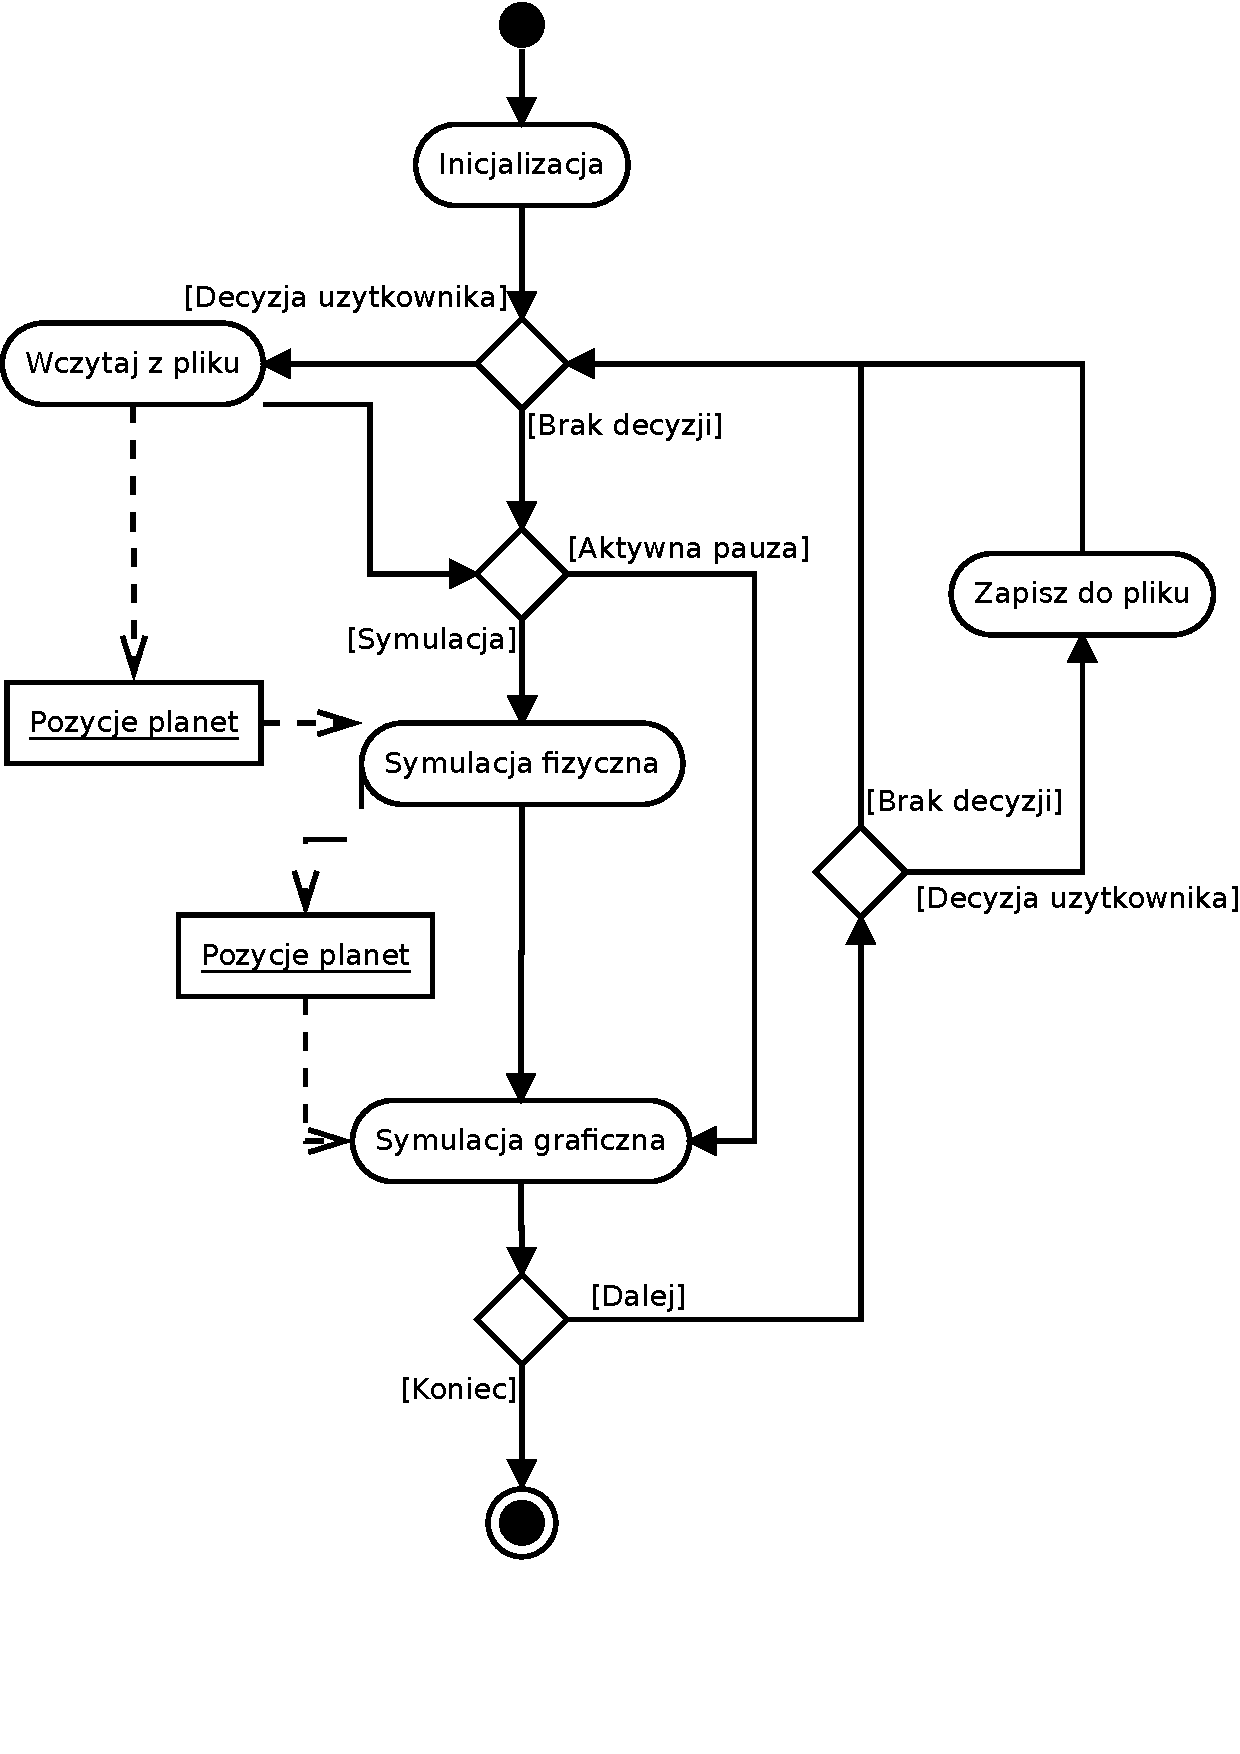
\includegraphics[width=0.75\textwidth]{activity.pdf}
	\caption{Diagram aktywności}
	\label{fig:activity}
\end{figure}


\begin{description}
	\item[Inicjalizacja aplikacji] \hfill \\
	Jest to pierwsza aktywność jaką wykonuje program. Składa się ona z inicjalizacji wszystkich modułów, w szczególności modułu graficznego i fizycznego. Zajmuje się także początkową alokacją pamięci i wczytaniem wszystkich potrzebnych zasobów, takich jak tekstury, modele oraz inne potrzebne dane.
	\item[Wczytanie z pliku] \hfill \\
	Jeśli użytkownik zdecyduje zacząć symulację z wcześniej przygotowanego pliku ta akcja jest za to odpowiedzialna. Musi ona załadować potrzebne dane z pliku oraz zapisać je poprzez pamięć RAM jednostki głównej do pamięci RAM jednostki graficznej. Użytkownik może również zdecydować o wczytaniu z pliku podczas już trwającej symulacji. W takim przypadku konieczne jest również zadbanie o odpowiednie wyczyszczenie poprzedniej symulacji, tak aby żadne artefakty nie zostały w pamięci RAM, zarówno jednostki głównej, jak i graficznej.
	\item[Zapis do pliku] \hfill \\
	Na życzenie użytkownika aktualny stan symulacji może zostać zapisany do pliku. W takim przypadku zbierane z aplikacji są wszystkie potrzebne dane, takie jak pozycje planet, wielkości i ciężary planet, modele planet, pozycja kamery itp. oraz zapisywane są do pliku.
	\item[Aktywna pauza] \hfill \\
	Symulacja wspiera tak zwaną "aktywną pauzę". Oznacza to, że na żądanie użytkownika symulacja fizyczna jest zatrzymana, natomiast cały czas reszta aplikacji jest w pełni funkcjonalna. Oznacza to, że można sterować kamerą, wczytywać/zapisywać układy planetarne oraz dodawać/usuwać planety.
	\item[Symulacja fizyczna] \hfill \\
	Jest to kluczowy moduł dla działania aplikacji. Podczas każdej takiej aktywności obliczane są kolejne pozycje planet do wyświetlenia. W jednej iteracji może być obliczona więcej niż jedna klatka fizyczna, jeśli moc obliczeniowa komputera na to pozwala.
	\item[Symulacja graficzna] \hfill \\
	Ta aktywność odpowiedzialna jest przede wszystkim za wyświetlanie symulacji na ekranie. Głównym jej zadaniem jest wyświetlanie planet na ich pozycjach wraz z towarzyszącymi im efektami graficznymi. Pozycje planet do wyświetlenia pobierane są z modułu fizycznego. Jeśli natomiast włączona jest aktywna pauza i nowe pozycje nie zostały wygenerowane, moduł korzysta ze starych pozycji. Po zakończonej jednej iteracji pętli, aplikacja odczekuje chwilę, żeby nie zajmować całego procesora oraz żeby zapewnić takie samo działanie symulacji na słabszych komputerach (gdzie czekanie może zostać pominięte)
\end{description}

\subsection{Struktura klas}\label{sub:struktura klas}
\paragraph{}
Ze względu na architekturę aplikacji, klasy używane na CPU oddzielone są od klas karty graficznej. Oczywiście te drugie są klasami jedynie logicznie - ze względu na konieczność używania języka C w kodzie dla GPU. Jednak ze względu na to, że obiekty są wygodną abstrakcją, będziemy z niej korzystać w całym programie.

\subsubsection{Klasy GPU}

\begin{figure}[h]
	\centering
	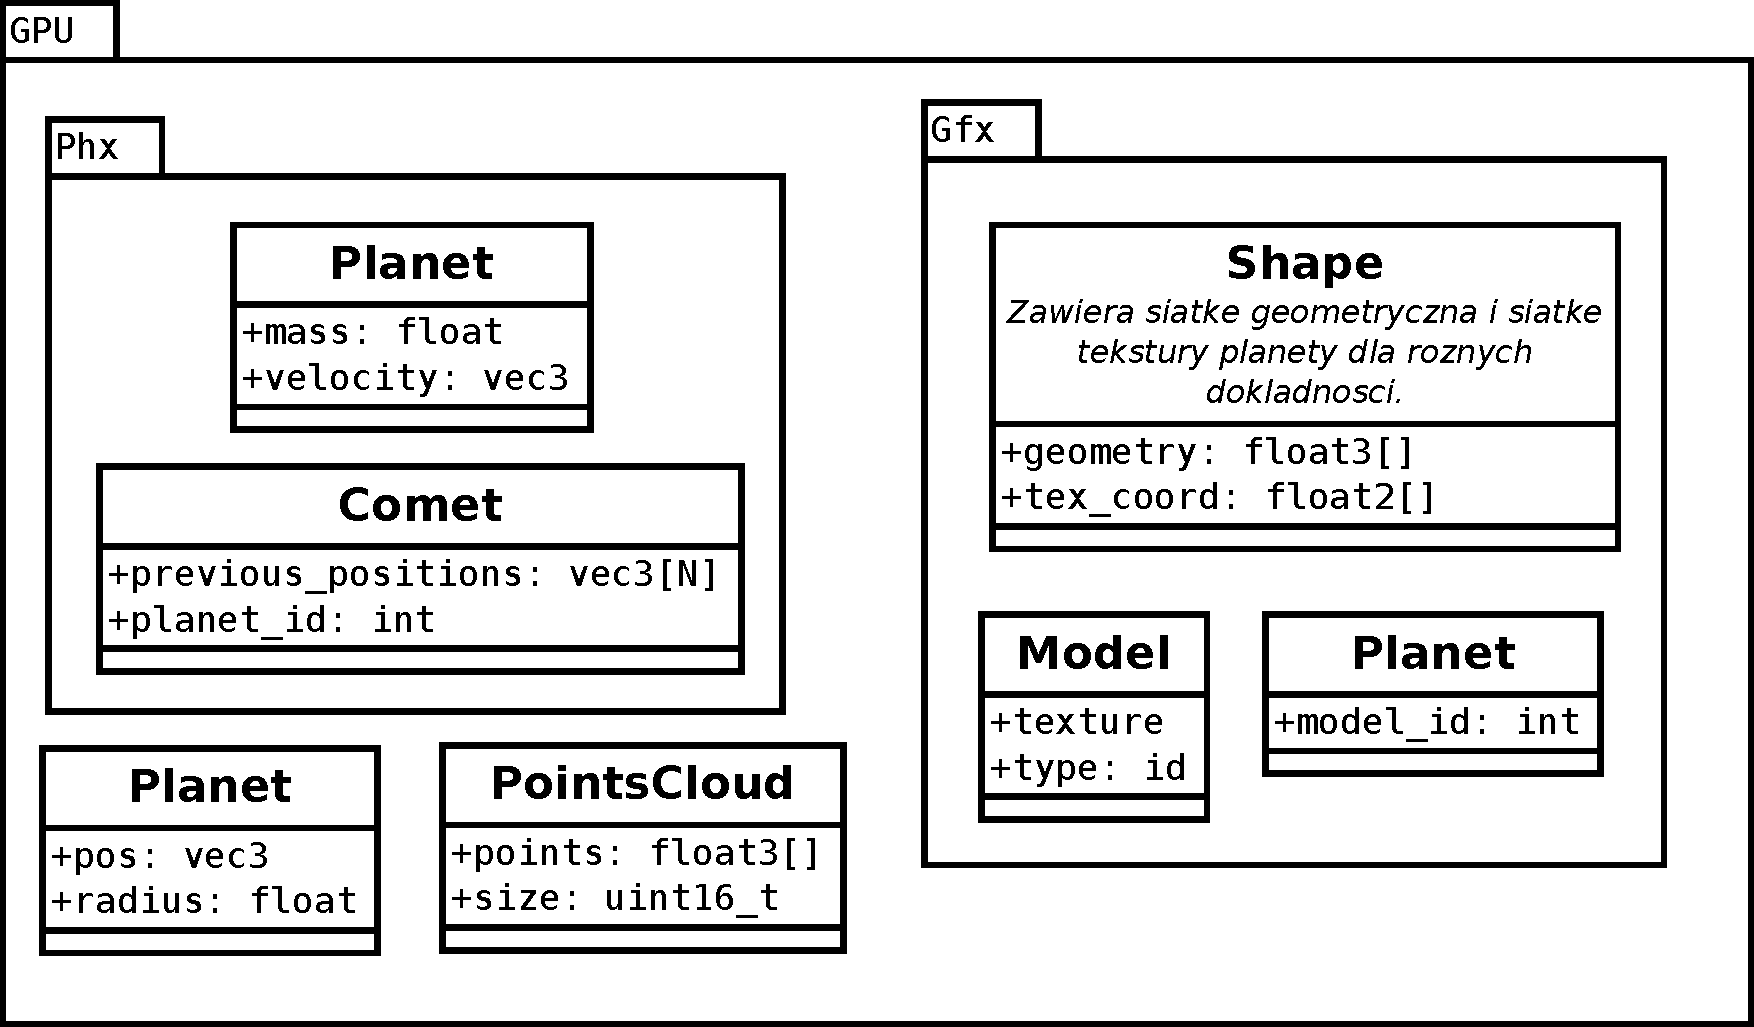
\includegraphics[angle=0,width=0.8\textwidth]{img/class_gpu.pdf}
	\caption{Diagram klas dla GPU}
	\label{fig:class_gpu}
\end{figure}

\paragraph{}
Struktury, z których będziemy korzystać na karcie graficznej, określone są na rysunku \ref{fig:class_gpu}. Ponieważ karta graficzna służy nam zarówno do wyświetlania danych, jak i do ich przetwarzania, wydzielone są na nim dwie przestrzenie nazw. Są to:
\begin{itemize}
	\item{Phx - do operacji fizycznych}
	\item{Gfx - do operacji graficznych}
\end{itemize}

\paragraph{}
Ponadto istnieje kilka struktur wspólnych dla obu częsci.

\begin{description}
\item{\bf GPU::Planet} zawiera informacje, z których korzystają zarówno wyświetlanie jak i fizyka. Jest to położenie planety oraz jej promień.
\item{\bf GPU::PointsCloud} reprezentuje chmurę cząstek - jest ona obliczana dla każdej widocznej komety przez moduł fizyczny.
\end{description}

\paragraph{}

Operacje fizyczne odbywać się będą z wykorzystaniem dwóch dodatkowych struktur.

\begin{description}
\item{\bf GPU::Phx::Planet} to dodatkowe informacje o każdej planecie, które są potrzebne jedynie silnikowi fizycznemu. Należą do nich prędkość oraz masa.
\item{\bf GPU::Phx::Comet} stanowi dodatkową informację o planecie. Struktura ta istnieje tylko dla obiektów będących kometami. Zawiera kilka ostatnich pozycji oraz identyfikator planety.
\end{description}

\paragraph{}

Do wyświetlenia planet konieczne będą informacje o teksturach oraz o siatkach każdej z planet.

\begin{description}
\item{\bf GPU::Gfx::Planet} zawiera indeks modelu, czyli wyglądu planetu. Dwie planety mogą mieć ten sam model.
\item{\bf GPU::Gfx::Model} definiuje konkretny wygląd. Na tym poziomie będziemy rozróżniać zwykłe planety od gwiazd i komet.
\item{\bf GPU::Gfx::Shape} agreguje informację o siatce planety w 3D oraz odpowiadającej jej siatce na dwuwymiarowej teksturze.
\end{description}

\subsubsection{Klasy CPU}

\begin{figure}[ht!]
	\centering
	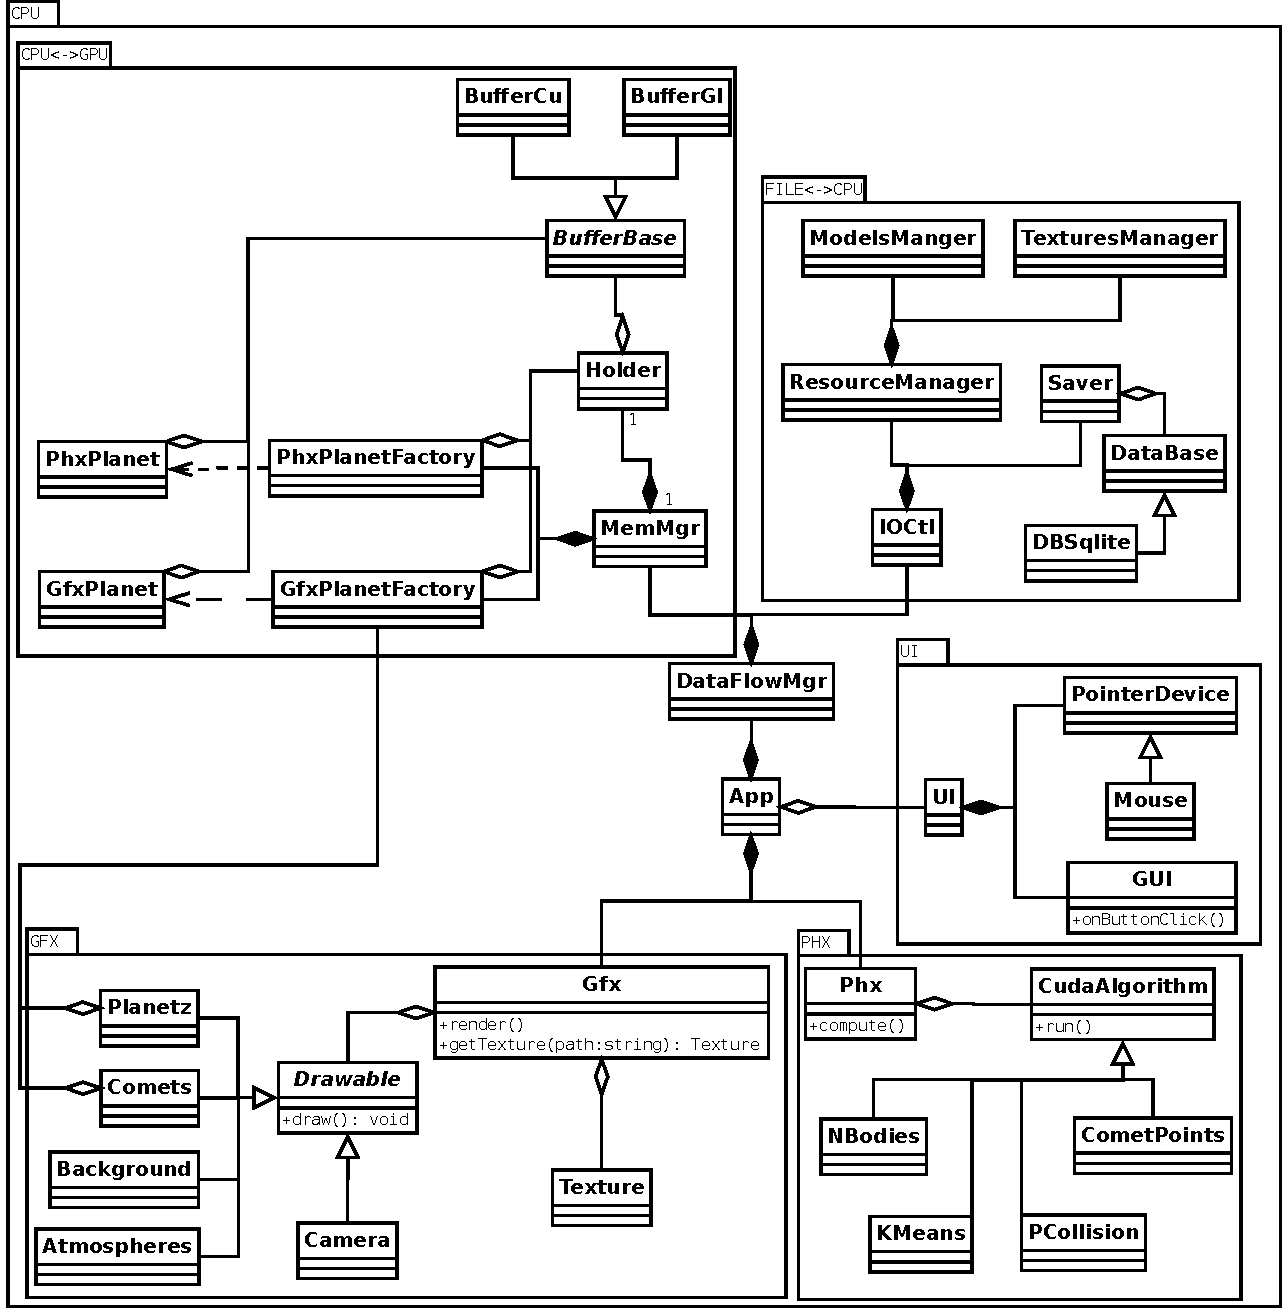
\includegraphics[angle=0,width=\textwidth]{img/class_cpu.pdf}
	\caption{Diagram klas dla CPU}
	\label{fig:class_cpu}
\end{figure}

\paragraph{}
Ta część klas przełoży się bezpośrednio na klasy znane z c++. Diagram klas znajduje się na rysunku \ref{fig:class_cpu}.

\begin{description}
\item{\bf CPU::App} jest główną klasą, zarządzającą obiektami GFX, PHX, DataFlowMgr oraz UI. Tworzy je ona na początku działania programu.
\item{\bf CPU::DataFlowMgr} wykonuje wszystkie przepływy danych - pomiędzy RAM karty graficznej, RAM komputera oraz dyskiem twardym.
\item{}
\item{\bf CPU::PHX::Phx} zarządza wykonaniem algorytmów wykonywanych na karcie graficznej.
\item{\bf CPU::PHX::CudaAlgorithm} abstrakcyjna klasa reprezentująca algorytm karty graficznej. Jeden algorytm może składać się z wywołań kilku kerneli CUDA.
\item{\bf CPU::PHX::NBodies} podstawowy algorytm w projekcie - wyliczenie oddziaływań planet między sobą.
\item{\bf CPU::PHX::KMeans} algorytm liczenia klastrów. W wersji podstawowej - standardowy algorytm k-means.
\item{\bf CPU::PHX::PCollision} algorytm wykrywający kolizje między planetami. W wersji podstawowej - uwzględnia jedynie kolizje wewnątrz klastrów.
\item{\bf CPU::PHX::CometPoints} obliczenie chmury punktów, służących do wyświetlenia ogona komety.
\item{}
\item{\bf CPU::GFX::Gfx} odpowiada za wyświetlanie wszystkich obiektów obecnych w przestrzeni 3D. Korzysta przy tym z biblioteki OpenGL.
\item{\bf CPU::GFX::Drawable} abstrakcja dla wszystkich obiektów, które chcą być wyświetlane.
\item{\bf CPU::GFX::Texture} obiekt tekstury, generowany przez klasę Gfx na podstawie bitmapy. Można zapobiec zbędnemu ładowaniu tekstur. Każda klasa, aby dostać taki obiekt, musi poprosić o niego klasę Gfx, która albo zwróci załadowaną teksturę, albo stworzy nowy obiekt tej klasy.
\item{\bf CPU::GFX::Planetz} obiekt wyświetlający wszystkie planety obecne na scenie.
\item{\bf CPU::GFX::Comets} obiekt wyświetlający wszystkie komety.
\item{\bf CPU::GFX::Background} wyświetla tło.
\item{\bf CPU::GFX::Atmospheres} klasa odpowiedzialna za wyświetlanie efektów atmosferycznych nad planetami.
\item{}
\item{\bf CPU::UI::UI} odpowiada za całość interakcji z użytkownikiem, czyli za obsługę zdarzeń myszki, klawiatury oraz graficzny interfejs użytkownika.
\item{\bf CPU::UI::GUI}, czyli graficzny interfejs użytkownika. Składać sie na to będą okna oraz guziki zagnieżdżone w oknie głównym aplikacji.
\item{\bf CPU::UI::PointerDevice} abstrakcja dla wszystkich wejściowych urządzeń, które mogą być wskaźnikami. W danej aplikacji będzie to najprawdopodobniej myszka, jednak takie podejście umożliwia dodanie obsługi takich peryferii jak dżojstiki czy kontrolery gier.
\item{\bf CPU::UI::Mouse} implementacja abstrakcji wskaźnika z użyciem myszki.
\item{}
\item{\bf CPU::FILE2CPU::IOCtl} klasa bazowa modułu odpowiedzialnego za wczytywanie danych z plików do pamięci ram oraz zapisywanie zmodyfikowanych danych do pliku.
\item{\bf CPU::FILE2CPU::ResourcesManager} klasa odpowiedzialna za zarządzenie zasobami aplikacji, takimi jak modele, tekstury i wszelkie inne dane przechowywane na dysku.
\item{\bf CPU::FILE2CPU::ModelsManager} służy do wczytywania modeli planet z dysku do pamięci RAM.
\item{\bf CPU::FILE2CPU::TexturesManager} służy do wczytywania tekstur do bitmap w pamięci RAM.
\item{\bf CPU::FILE2CPU::DataBase} abstrakcyjna klasa służąca do komunikacji aplikacji z bazą danych. Aplikacja będzie najprawdopodobniej korzystać z bazy sqlite, która jest idealna do takich zastosowań, jednak użycie abstrakcji pozwoli na bezbolesną podmianę bazy w razie konieczności.
\item{\bf CPU::FILE2CPU::DBSqlite} implementacja abstrakcji bazy danych do komunikacji z bazą sqlite.
\item{}
\item{\bf CPU::CPU2GPU::MemMgr} na zlecenie DataFlowMgr'a przenosi dane pomiędzy kartą graficzną a RAM.
\item{\bf CPU::CPU2GPU::Holder} Agreguje wszystkie bufory potrzebne do reprezentacji planety. Zarówno te fizyczne, graficzne, jak i wspólne.
\item{\bf CPU::CPU2GPU::BufferBase} bazowa, abstrakcyjna klasa dla buforów jednostki graficznej. Dzięki temu danymi dostępnymi dla programów jednostki graficznej można wygodnie manipulować z poziomu kodu jednostki centralnej.
\item{\bf CPU::CPU2GPU::BufferCu} reprezentuje dane przetrzymywane na karcie graficznej przy pomocy wywołań biblioteki CUDA.
\item{\bf CPU::CPU2GPU::BufferGl} reprezentuje dane przetrzymywane na karcie graficznej przy pomocy wywołań biblioteki OpenGL. Technologia CUDA pozwala na udostępnianie buforów opengla dla programów CUDA, dzięki temu bufor ten używany jest tam, gdzie potrzebny jest dostęp do danych zarówno z modułów graficznych, jak i fizycznych.
\item{\bf CPU::CPU2GPU::PhxPlanetFactory} jest faktorią dla obiektów reprezentujących planety z punktu widzenia fizyki na karcie graficznej.
\item{\bf CPU::CPU2GPU::GfxPlanetFactory} analogiczna klasa, ale tworząca obiekty graficzne.
\item{\bf CPU::CPU2GPU::PhxPlanet} obiekt zawierający bufory karty graficznej potrzebne do obliczeń fizycznych.
\item{\bf CPU::CPU2GPU::GfxPlanet} analogiczny do PhxPlanet, z tą różnicą, że posiada niemodyfikowalne bufory potrzebne do wyświetlania planet.
\end{description}

